\documentclass{article}
\usepackage{graphicx}
%pages setting
\usepackage{geometry}
\geometry{a4paper, centering, scale = 0.8}

\title{COMSM0104-Web Technologies Report}
\author{Kehan Du, Shunyi Zhao}

\begin{document}

\maketitle

\section{Introduction}
Our team is comprised of Kehan Du (mz19460) and Shunyi Zhao (vt19049). The
aim of our project is to construct the PC end official website of Deep KW
Innovation Factory.

~\\
\noindent
Deep KW Innovation Factory is the academic workshop of interdisciplinary 
at Huazhong University of Science and Technology, China. Since the establishment 
of Deep KW Innovation Factory in 2017, it has always upheld and practiced 
the concepts and methods of interdisciplinary, and insisted on exploring 
the question of social sciences by using natural science methods.

~\\
\noindent
The central goal of this version is to construct of the official website 
framework and the dynamic realization of key pages and complete the initial 
launch of the official website. This version is just used to practice the skills
of web technologies, and will not be used commercially. We have got the
permission to do this website, and the final report will declare the copyright.

\section{Page Design}
The home page of this project is shown below:
\\
\begin{figure}[h]
    \centering
    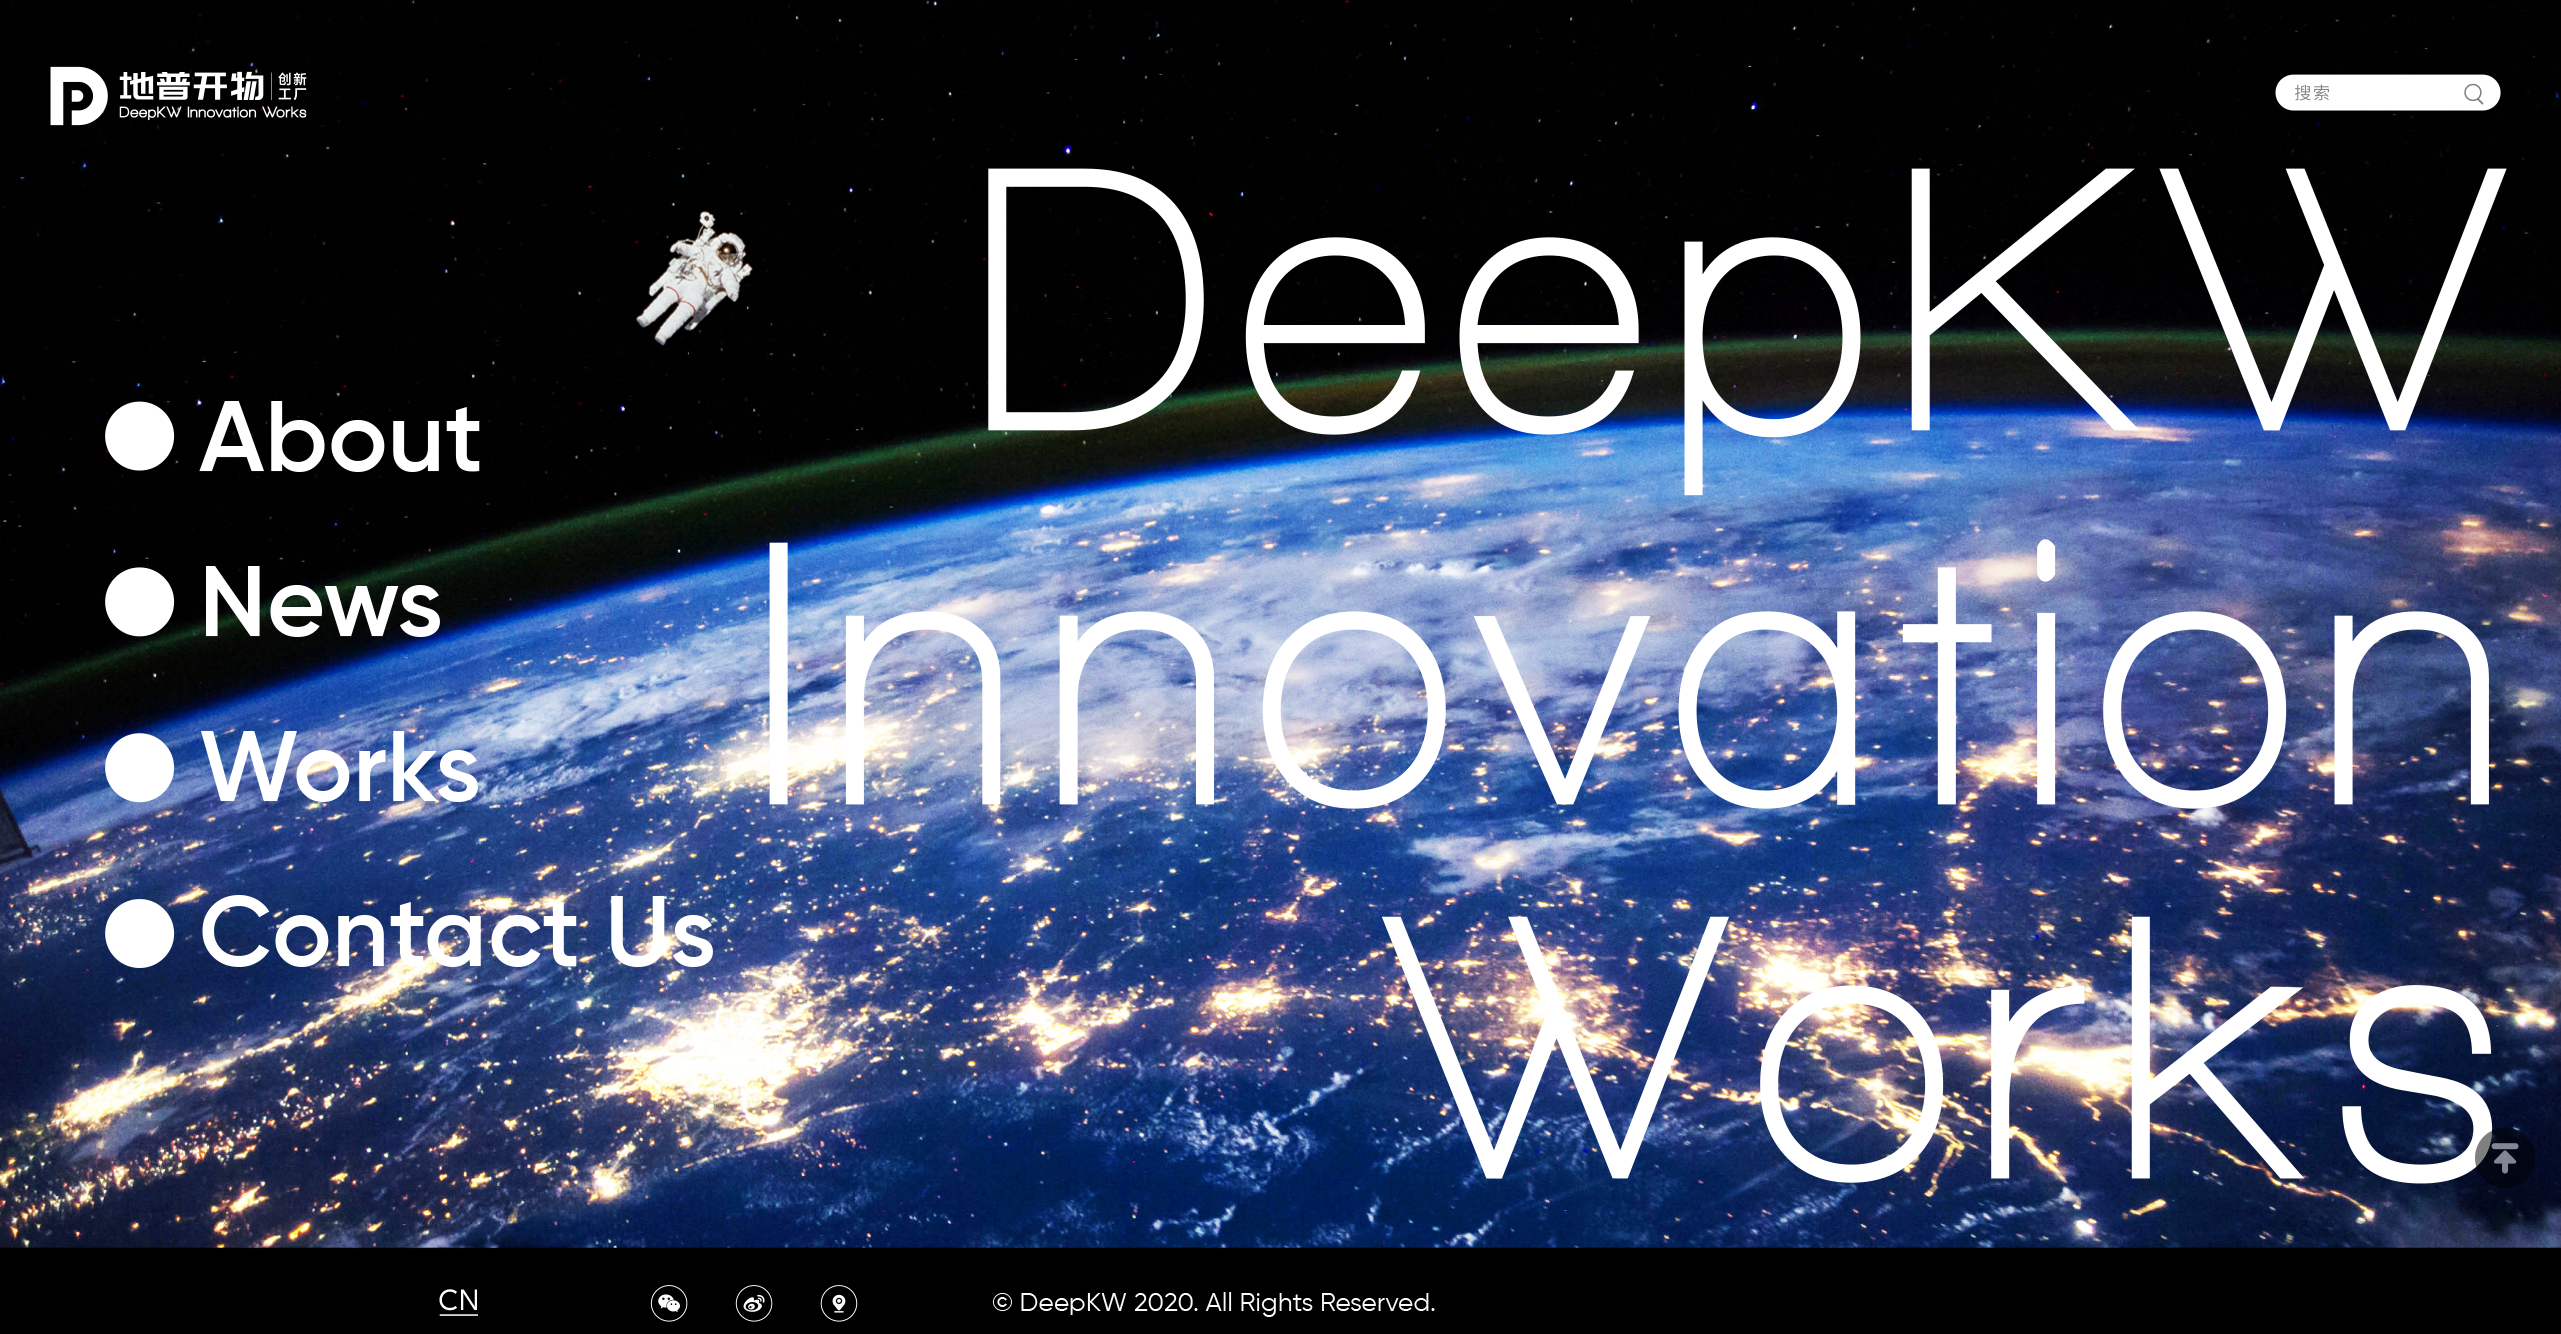
\includegraphics[height=4cm]{img/02.png}
    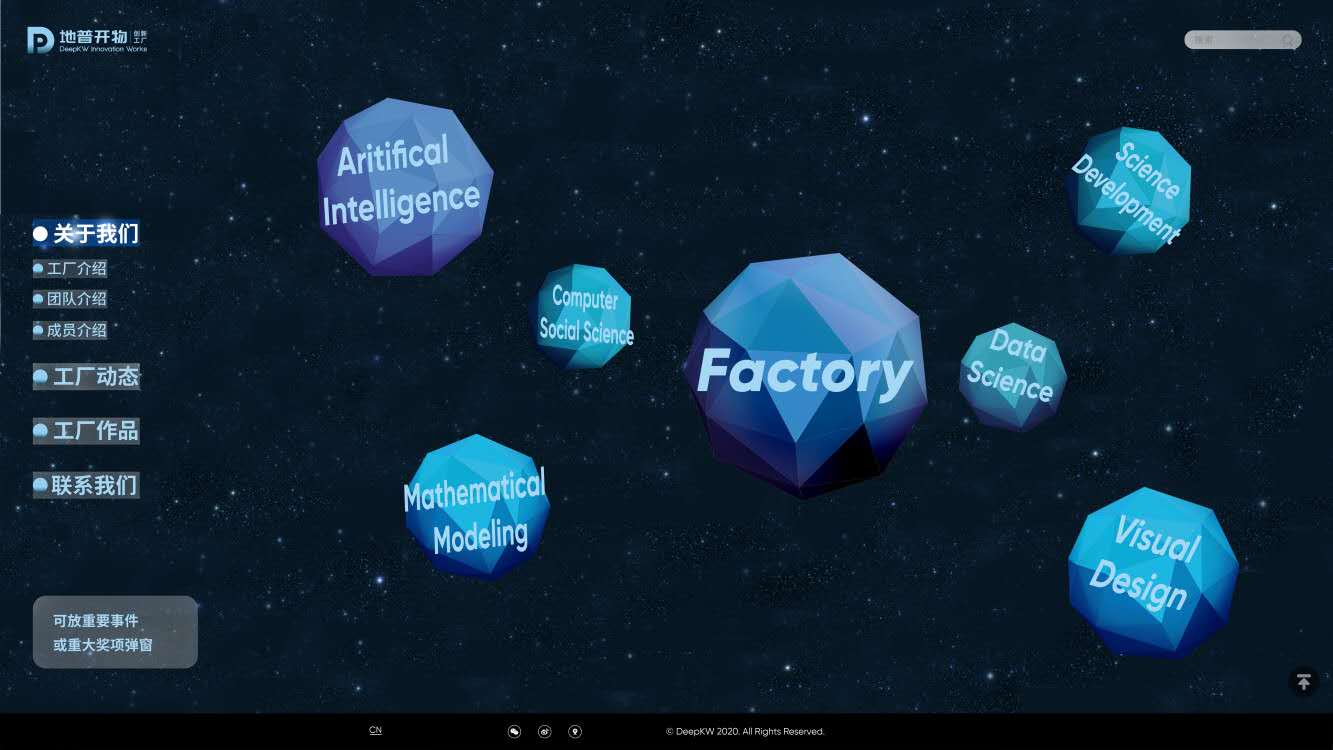
\includegraphics[height=4cm]{img/05.jpg}
    \caption{home page and about page}
    \label{fig: figure1}
\end{figure}
\\
\section{Technology Evaluation}
\subsection{Estimation of marks}
\begin{itemize}
    \item A for HTML
    \item A for CSS
    \item A for JS
    \item B for PNG
    \item B for SVG
    \item B for Server
    \item B for Database
    \item B for dynamic pages
    \item 12 for Depth (out of 20)
\end{itemize} 

\subsection{Client Side}
We chose a popular javascript framework, Vue.js (version 2.6.11), to 
develop these pages.
Modularity and componentization are important features of Vue,  
allowing us to build complex applications with small, independent, 
and usually reusable components. And these components convenient 
for later maintenance and upgrade of the official website. 
We use webpack and npm manage the packages based on node.js, and 
information about these packages is shown in package.json. Works are 
placed in folder named \textit{./src/components}. HTML, used as 
the template of every module, and CSS would control the layout 
and style of these modules.

~\\
\noindent
Adobe Photoshop and Illustrator (Authorized) are used to design the 
blueprint of the website, and some .png file are created by them. 
Some icons, such as the logo of group, are drawn by SVG.

\subsubsection{HTML}
HTML is an integral part of the Vue component demonstrated as ```<template>``` tag. 
Vue.js uses an HTML-based template syntax that allows programmers to declaratively 
bind the rendered DOM to the underlying Vue instance’s data. The advantage of Vue 
is it compiles the templates into Virtual DOM render functions. Combined with the 
reactivity system, Vue is able to intelligently figure out the minimal number of 
components to re-render and apply the minimal amount of DOM manipulations when the 
app state changes.

~\\
\noindent
In our project, only one index.html document is used as the entrance, which is 
accessed through index.js.Other pages are all broken down into components, 
which are stitched together like building blocks.Compared with basic .html 
document, Vue's template HTML reduces the replication of many HTML statements. 
At the same time, the grammar in the Vue framework makes the data no longer 
nested in HTML statements, making the project itself more flexible.

~\\
\noindent
In this project, BaseNav.vue (project/src/components/Common/BaseNav.vue) 
is a good example. This is a common Navigation component, which uses list 
rendering to render the navigation name(data) into HTML, and completes 
the task with a brief HTML statement.

\begin{figure}[h]
    \centering
    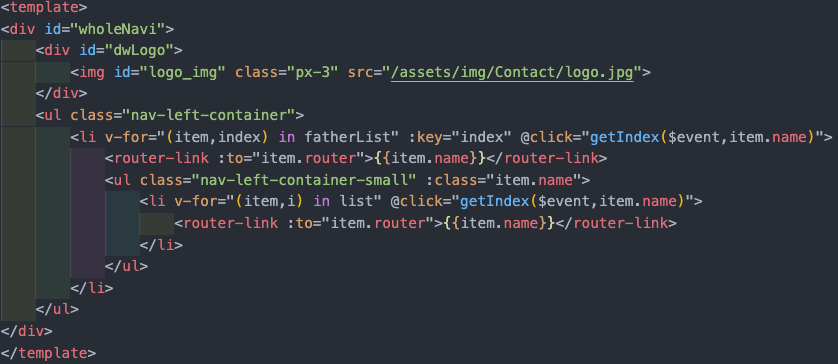
\includegraphics[width=13cm]{img/exp/html.png}
    \caption{The HTML codes written in BaseNav.vue}
    \label{}
\end{figure}
\subsubsection{CSS}
CSS is also an integral part of the Vue component demonstrated 
as \textless style\textgreater. The advantage is that the scope of CSS can be 
limited by adding the "scoped" attribute.

~\\
\noindent
Vue supports a variety of CSS, Less, Sass style expression mode, 
this project uses basic CSS for style editing. At the same time, 
we also carried out basic beautification of some HTML parts with 
the help of Bootstrap4. The use of Flexbox in the layout, 
this method effectively improves the website screen adaptability.

~\\
\noindent
Original CSS  can be reflected in groups.vue 
(project/src/components/About/groups.vue).Finally achieving the 
predetermined goal of the design diagram.

\begin{figure}[h]
    \centering
    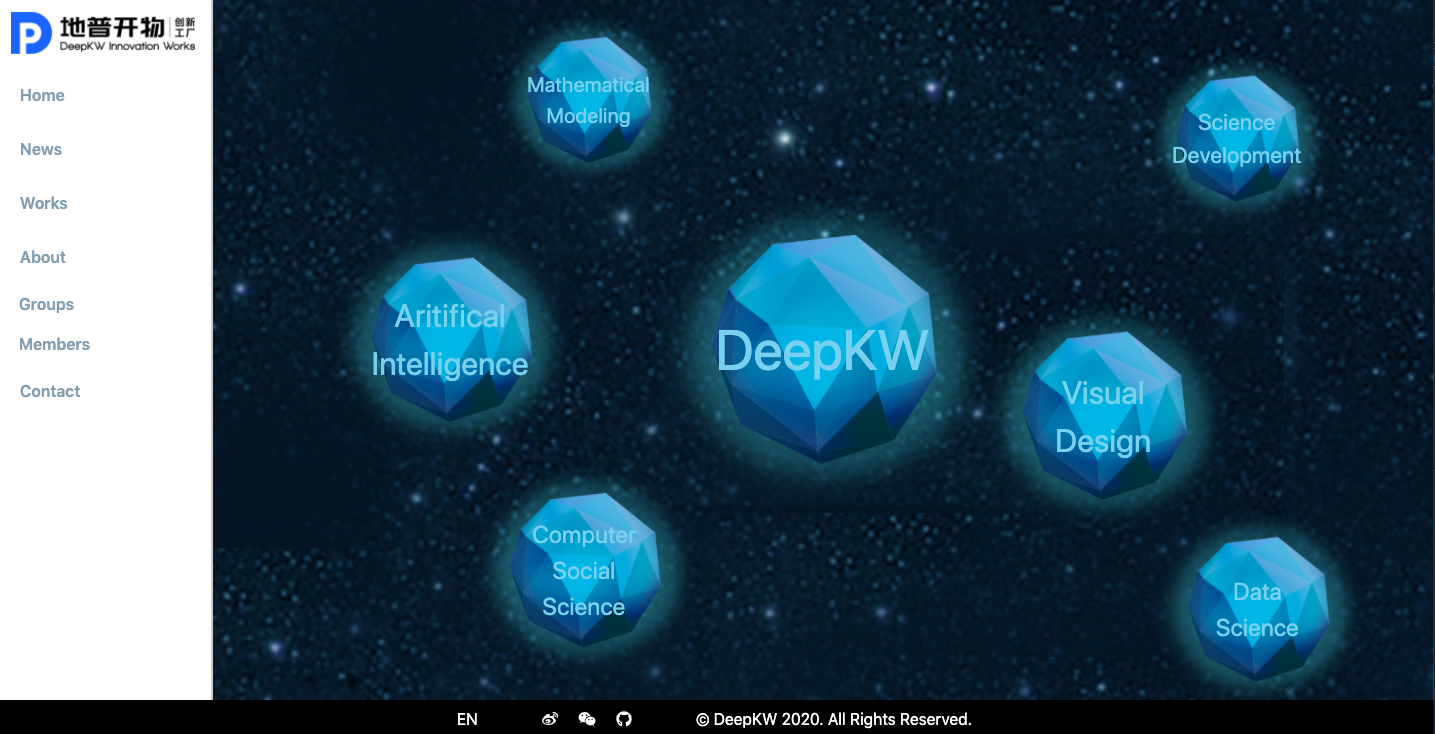
\includegraphics[width=10cm]{img/exp/css.png}
    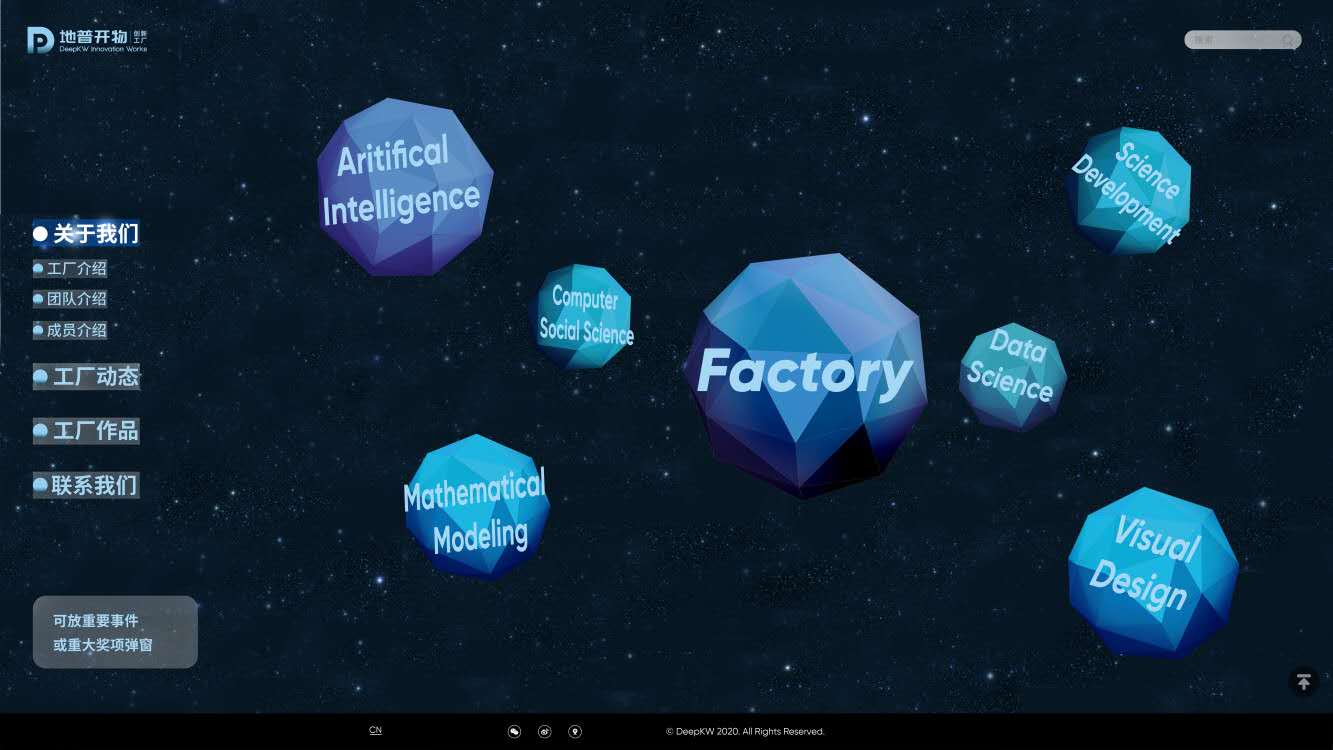
\includegraphics[width=10cm]{img/05.jpg}
    \caption{}
    \label{}
\end{figure}

\subsubsection{JavaScript}
\subsubsection{PNG}
Some images used in this project are drawn with GIMP 2. One of the examples,
textit{table.png} which is ued in \textit{Contact.vue}, is shown below in 
Figure \ref{fig: figure2}.

\begin{figure}[h]
    \centering
    
\includegraphics{img/sectionPNG/table2.png}
    
\includegraphics{img/sectionPNG/table1.png}
    \caption{Left: the image after adding three text objects. 
    Right: add three rectangles with 48.0 opaqueness.}
    \label{fig: figure2}
\end{figure}

\noindent
Firstly, we added three text objects into a $ 300 \times 400 $ file, and then 
typed in some useful information. Then the coverages of these text objects are
combined to fix the positions of them. The result of this stage is shown in the 
left image of Figure \ref{fig: figure2}. And then, three rectangular layers are 
added, the result is shown in the right image of Figure \ref{fig: figure2}. 



\subsubsection{SVG}

\subsection{Sever Side}
\subsubsection{Server}
The development of Sever is also in node.js. We use \textit{express} as the 
server framework.
\subsubsection{Database}
We choose \textit{sqlite3} to manage our databases. 
We use four tables, including candidata, , in this project.
The ER relationship of 
tables used in this project is shown below. 

\subsubsection{Dynamic Page}
A good example of dynamic page in our project is the \textit{Works} page.
We use a method called getAll() in the file
(project/src/components/Works/Selecter.vue). This method is also used in the 
created part of Vue, which could get the data of all the works stored in databases
when this webpage is initialized. The layout of this page is shown below in 
Figure 
    
\end{document}
